%% 
%% This is file, `6-g-rat.tex',
%% generated with the extract package.
%% 
%% Generated on :  2017/08/15,12:01
%% From source  :  readiness.tex
%% Using options:  active,generate=rat/6-G-RAT.tex,extract-env={readinessAssuranceTest}
%% 
\documentclass{article}
 \usepackage{tbil-la,course-notes}

\begin{document}

\begin{readinessAssuranceTest}

\item Find the area of the parallelogram with vertices $(0,0)$, $(4,0)$, $(5,2)$, and $(1,2)$.
\begin{multicols}{2}
\begin{readinessAssuranceTestChoices}
\item $5$
\item $6$
\item $7$
\item $8$
\end{readinessAssuranceTestChoices}


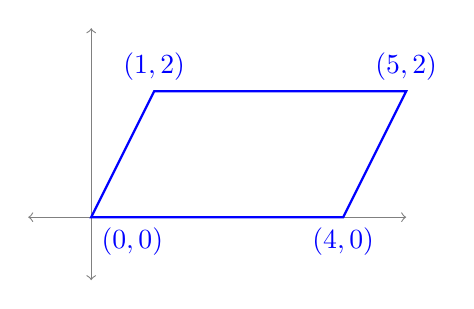
\begin{tikzpicture}[scale=0.8]
\draw[thin,gray,<->] (-1,0)-- (5,0);
\draw[thin,gray,<->] (0,-1)-- (0,3);
\draw[thick,blue] (0,0) node[below right] {$(0,0)$} -- (4,0)node [below] {$(4,0)$} -- (5,2) node[above] {$(5,2)$} -- (1,2) node[above]{$(1,2)$} -- cycle;
\end{tikzpicture}
\end{multicols}

\item Find the area of the parallelogram with vertices $(0,0)$, $(12,5)$, $(14,8)$, and $(2,3)$.
\begin{multicols}{2}
\begin{readinessAssuranceTestChoices}
\item $13$
\item $26$
\item $39$
\item $52$
\end{readinessAssuranceTestChoices}


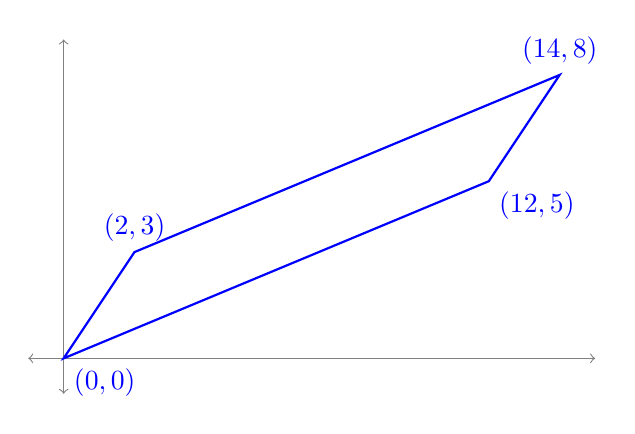
\begin{tikzpicture}[scale=0.45]
\draw[thin,gray,<->] (-1,0)-- (15,0);
\draw[thin,gray,<->] (0,-1)-- (0,9);
\draw[thick,blue] (0,0) node[below right] {$(0,0)$} -- (12,5)node [below right] {$(12,5)$} -- (14,8) node[above] {$(14,8)$} -- (2,3) node[above]{$(2,3)$} -- cycle;
\end{tikzpicture}
\end{multicols}

\item The parallelogram ABCD has area $6$.  If AE is $\frac{3}{2}$ the length of AB, what is the area of the parallelogram AEFD?
\begin{multicols}{2}
\begin{readinessAssuranceTestChoices}
\item $9$
\item $12$
\item $15$
\item $18$
\end{readinessAssuranceTestChoices}

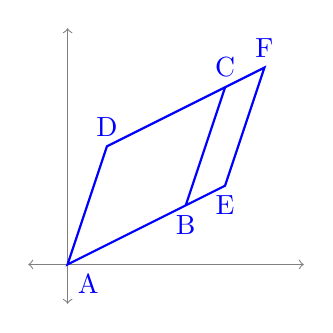
\begin{tikzpicture}[scale=0.5]
\draw[thin,gray,<->] (-1,0)-- (6,0);
\draw[thin,gray,<->] (0,-1)-- (0,6);
\draw[thick,blue] (0,0) node[below right] {A} --(4,2) node[below] {E} -- (5,5) node[above]{F} -- (1,3)node[above] {D} -- cycle;
\draw[thick,blue] (3,1.5) node[below] {B} -- (4,4.5) node [above] {C};
\end{tikzpicture}
\end{multicols}

\item The parallelogram ABCD has area $6$.  If AF is one third as long as AD, what is the area of the parallelogram ABEF?
\begin{multicols}{2}
\begin{readinessAssuranceTestChoices}
\item $1$
\item $2$
\item $3$
\item $4$
\end{readinessAssuranceTestChoices}

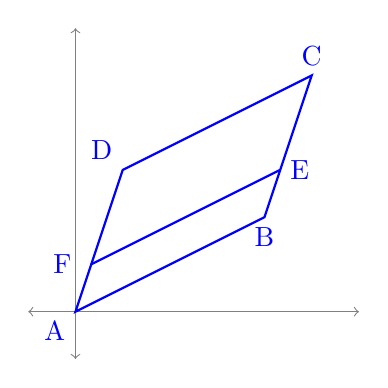
\begin{tikzpicture}[scale=0.6]
\draw[thin,gray,<->] (-1,0)-- (6,0);
\draw[thin,gray,<->] (0,-1)-- (0,6);
\draw[thick,blue] (0,0) node[below left] {A} --(4,2) node[below] {B} -- (5,5) node[above]{C} -- (1,3)node[above left] {D} -- cycle;
\draw[thick,blue] (0.33,1) node[left] {F\ \ } -- (4.33,3) node [right] {E};
\end{tikzpicture}
\end{multicols}

\item Let $T: \IR^2 \rightarrow \IR$ be a linear transformation.  Which of the following is equal to $T\left(\begin{bmatrix} a+b \\ a+b \end{bmatrix}\right)$?
\begin{multicols}{2}
\begin{readinessAssuranceTestChoices}
\item $T\left(\begin{bmatrix}a \\ b \end{bmatrix} \right)$
\item $2T\left(\begin{bmatrix}a \\ b \end{bmatrix} \right)$
\item $T\left(\begin{bmatrix}a \\ b \end{bmatrix} \right)+T\left(\begin{bmatrix}b \\ a \end{bmatrix} \right)$
\item $T\left(\begin{bmatrix} a \\ a \end{bmatrix}\right)+T\left(\begin{bmatrix}a \\ b \end{bmatrix} \right)+T\left(\begin{bmatrix}b \\ a \end{bmatrix}\right)+T\left(\begin{bmatrix}b \\ b \end{bmatrix} \right)$
\end{readinessAssuranceTestChoices}
\end{multicols}

\item Let $T: \IR^n \rightarrow \IR^n$ be a linear transformation with associated matrix $A \in M_n(\IR)$.  Three of the four answer choices are equivalent to each other; which one is not equivalent to the other three?\begin{readinessAssuranceTestChoices}
\item $A$ is not an invertible matrix
\item $T$ has a non-trivial kernel
\item $\det(A)\neq 0$
\item $A\vec{x}=\vec{b}$ has multiple solutions for all $\vec{b} \in \IR^n$.
\end{readinessAssuranceTestChoices}

\item What is the matrix corresponding to the linear transformation $T: \IR^3 \rightarrow \IR^3$ given by $T\left( \begin{bmatrix} x \\ y \\ z \end{bmatrix}\right) = \begin{bmatrix} 3x+2y-z \\ y+z \\x+7z \end{bmatrix}$?
\begin{multicols}{4}
\begin{readinessAssuranceTestChoices}
\item $\begin{bmatrix} 3 & 2 & -1 \\ 0 & 1 & 1 \\ 1 & 0 & 7  \end{bmatrix}$
\item $\begin{bmatrix} 3 & 0 & 1 \\ 2 & 1 & 0 \\ -1 & 1 & 7 \end{bmatrix}$
\item $\begin{bmatrix} 3 & 2 & -1 \\ 1 & 1 & 0 \\ 1 & 7 & 0 \end{bmatrix}$
\item $\begin{bmatrix}  3 & 1 & 1 \\ 2 & 1 & 7 \\ -1 & 0 & 0 \end{bmatrix}$
\end{readinessAssuranceTestChoices}
\end{multicols}

\item Which of the following conditions imply that the quadratic polynomial $ax^2+bx+c$ has no real roots?
\begin{readinessAssuranceTestChoices}
\item $a<0$
\item $b^2-4ac<0$
\item $ac-b^2<0$
\item $ab+c^2<0$
\end{readinessAssuranceTestChoices}

\item Which of the following is a root of the polynomial $x^2-4x+13$?
\begin{multicols}{4}
\begin{readinessAssuranceTestChoices}
\item $1+2i$
\item $2-3i$
\item $3+4i$
\item $4-5i$
\end{readinessAssuranceTestChoices}
\end{multicols}

\item How many roots does the polynomial $x^4+3x^3+x^2-3x-2$ have?
\begin{multicols}{4}
\begin{readinessAssuranceTestChoices}
\item $1$
\item $2$
\item $3$
\item $4$
\end{readinessAssuranceTestChoices}
\end{multicols}

\end{readinessAssuranceTest}

\end{document}
